% !TEX root = ../main.tex

\section{Design History and Decisions}
\label{sec:design-history}

\scaffold{
  \textbf{Paragraph 1, purpose of the section.} The hardware went through four stages: the project proposal (April 2026) \cite{benson2026proposal}, the circuit of milestone~1, a breadboard prototype (August 2026) and the final PCB (designed late August to early September 2026, assembled end of September). \Cref{tab:design-history} compares them; the following paragraphs give the reason for every change. The reader should finish the section knowing why the final board looks as it does, so that \crefrange{sec:analog-front-end}{sec:pcb} can describe it without justifying it again. Write in the past tense (events of the project), as the writing guide prescribes for findings.
}

\begin{table}[htbp]
  \centering
  \small
  \titledcaption{Design Stages}{\scaffoldinline{Explain the four columns (proposal \cite{benson2026proposal}, milestone~1 circuit, breadboard prototype, final PCB) and that the text gives the reason for each change. Cells marked [?] are unconfirmed.}}
  \label{tab:design-history}
  \begin{tabularx}{\linewidth}{@{}>{\raggedright\arraybackslash}p{0.15\linewidth}*{4}{>{\raggedright\arraybackslash}X}@{}}
    \toprule
    & \textbf{Proposal} & \textbf{Milestone 1} & \textbf{Breadboard} & \textbf{Final PCB} \\
    \midrule
    Microcontroller & STM32G4 or RP2040 & Pico~2 module & Pico~2~W & Pico~2~W \\
    ADC & ADS8688, 16-bit SAR & AD7124-8, 24-bit $\Sigma\Delta$ & AD7718 [?] & 2$\times$ AD7718, 24-bit $\Sigma\Delta$ \\
    Pull switching & TS5A23157 SPDT switches & SN74LVC126A tristate buffers & tristate buffers [?] & TMUX1511 SPST switches \\
    Pull resistance & series resistor per contact & \qty{1}{\kilo\ohm} per contact & \qty{1}{\kilo\ohm} per contact & \qty{1}{\kilo\ohm} \qty{0.1}{\percent}, shared per rail and jack \\
    Input filter & RC & \qty{1}{\kilo\ohm}, \qty{100}{\nano\farad} & \qtyrange{68}{100}{\nano\farad} [?] & \qty{10}{\kilo\ohm}, \qty{10}{\nano\farad} \\
    Contacts per jack & 3 & 4 (one unused) & 3 & 4 (tip switch used) \\
    Analog rail, reference & separate analog rail & \qty{3.3}{\volt} analog rail & \qty{3.3}{\volt} & \qty{2.5}{\volt} LDO, pull-up rail and reference \\
    Ground & star point & star point & -- & one ground net \\
    Outputs & USB MIDI, optional DIN MIDI & USB MIDI & USB MIDI, WiFi & USB MIDI, WiFi, 4 LEDs \\
    \bottomrule
  \end{tabularx}
\end{table}

\begin{figure}[htbp]
  \centering
  \begin{subfigure}[t]{\linewidth}
    \centering
    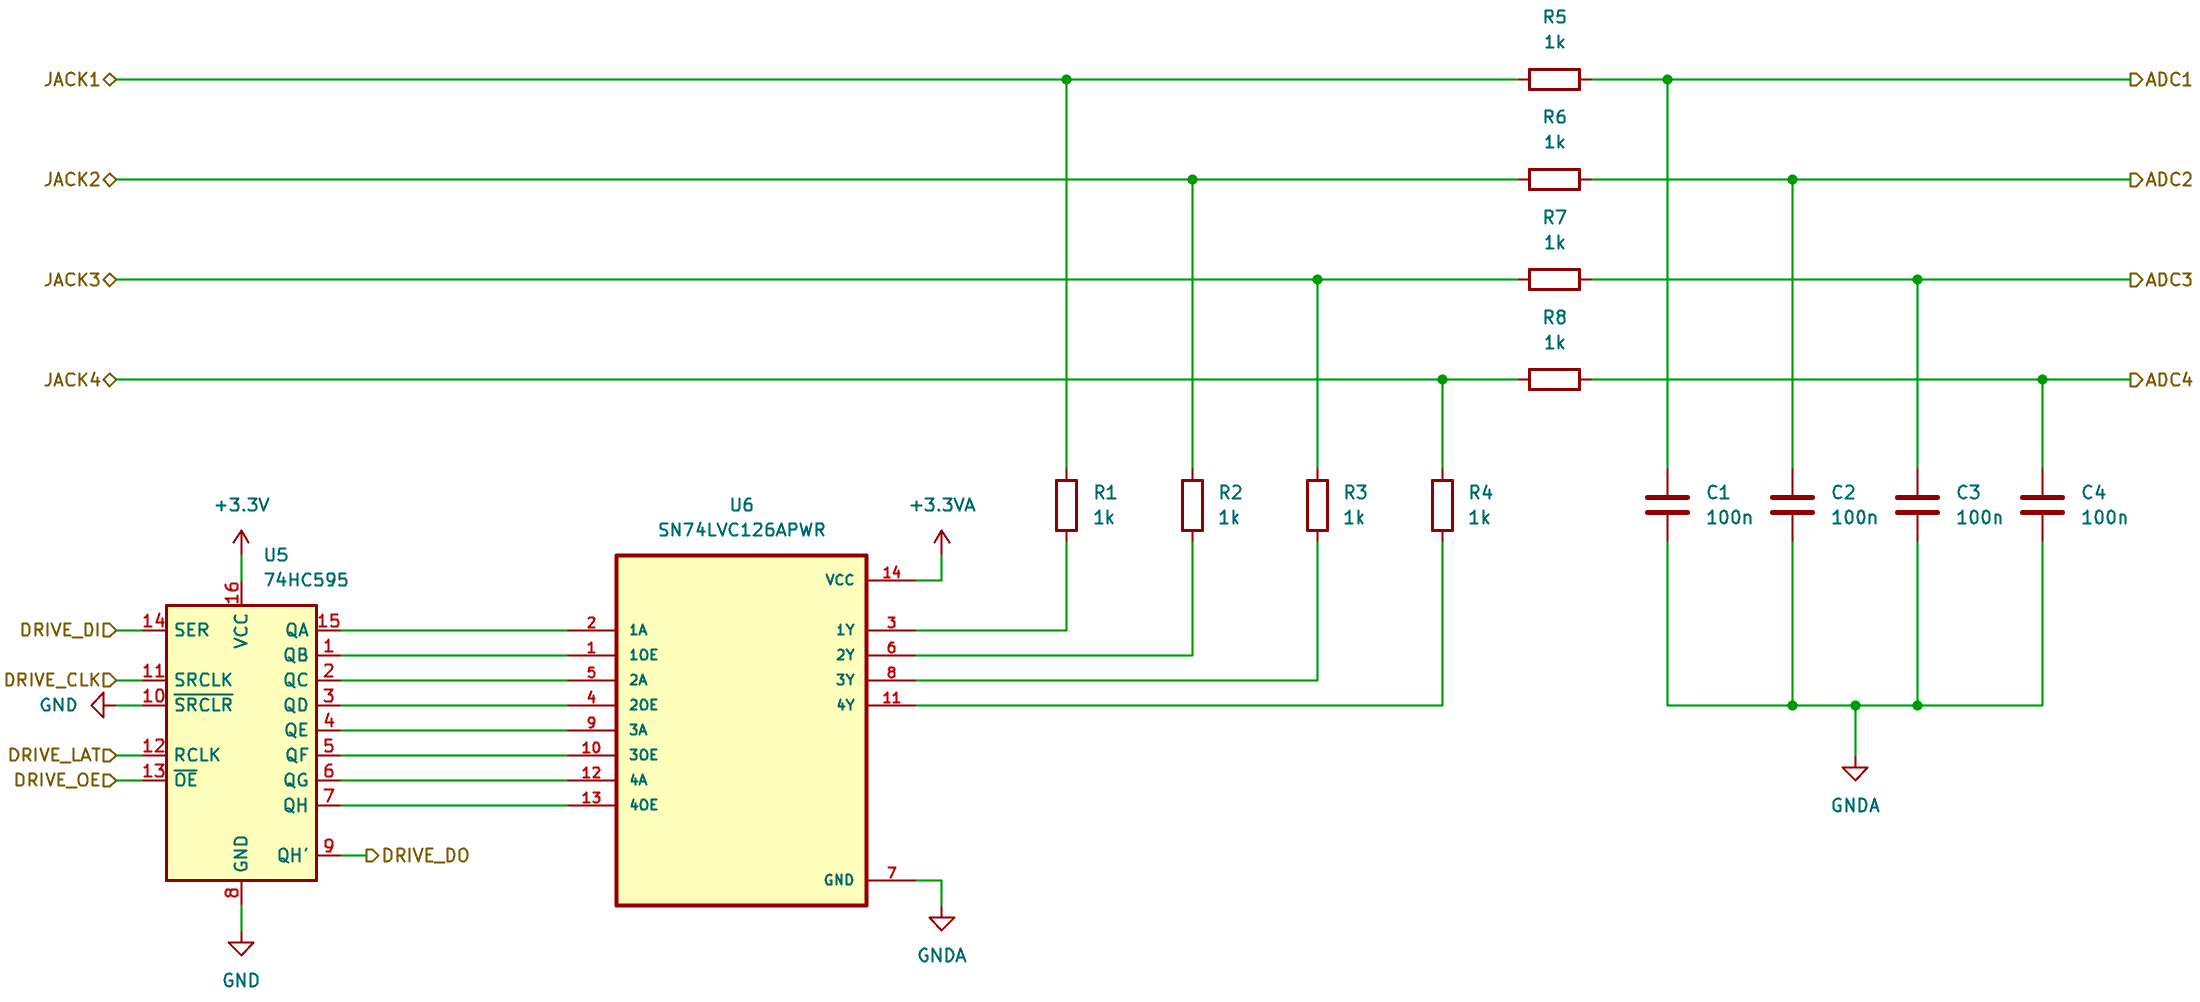
\includegraphics[width=0.85\linewidth]{04-implementation/figures/frontend-milestone-1}
    \caption{Milestone 1: Tristate Buffers}
    \label{fig:frontend-milestone-1}
  \end{subfigure}

  \vspace{4mm}
  \begin{subfigure}[t]{\linewidth}
    \centering
    \placeholderfigure[0.85\linewidth]{
      \textbf{Content.} The pull stage of one jack of the final board, cropped from \cref{fig:frontend-final}: U6 (74HC595), U15 and U19 (TMUX1511) with the shared resistors R50 and R54, without the RC filters.
      \textbf{Focus.} Same scale and orientation as (a), so that buffer and switch versions can be compared directly.
      \textbf{How to obtain.} Crop \code{04-implementation/figures/frontend-final.png} or export the sheet \code{hardware/AnalogQuadChannel.kicad\_sch} with \code{kicad-cli sch export svg}.
    }
    \caption{Final PCB: Analog Switches}
    \label{fig:frontend-switches}
  \end{subfigure}
  \titledcaption{Pull Stage Before and After the Change}{\scaffoldinline{(a): each 74HC595 output pair drives data and output enable of one SN74LVC126A buffer, whose output reaches the contact through a \qty{1}{\kilo\ohm} resistor (R1--R4); R5--R8 and C1--C4 form the old filter. (b): one switch per contact and rail, all switches of a rail sharing one \qty{0.1}{\percent} resistor.}}
  \label{fig:pull-stage-history}
\end{figure}

\subsection*{Pull Switching}

\scaffold{
  Proposal: SPDT analog switches \cite{ti2026ts5a23157}. Milestone~1 and breadboard: tristate buffers (SN74LVC126A \cite{ti2026sn74lvc126a}) driven by a 74HC595 chain, two control bits per contact (data and output enable), with a \qty{1}{\kilo\ohm} resistor at each output (\cref{fig:frontend-milestone-1}). Reason for the change to TMUX1511 switches \cite{ti2025tmux1511} (author's statement in the final presentation): the buffers worked in most cases, but their output impedance is only specified as a range and changed with the applied voltage, while the current computation of \cref{eq:currents} needs a precisely known pull resistance. The on-resistance of the switches, about \qty{2}{\ohm}, is negligible against the \qty{1}{\kilo\ohm} resistor, and \qty{0.1}{\percent} resistors make the pull resistance a known quantity. Add the consequence that comes for free: because the switches of one rail share one resistor, only one contact per rail can be driven at a time, which is exactly the one-high-one-low pattern of \cref{sec:pair-measurement}. Date of the change: 30~August~2026, which required a new schematic and a new layout.
}

\openquestion{Breadboard parts}{
  Which ADC and which buffer IC did the breadboard prototype use? The firmware drove an AD7718 from 6~August~2026, the parts list of the prototype names an ADS1241 and SN74LVC126A, and one development session refers to \enquote{74HC125-type} buffers. Also confirm the capacitance at each contact of the breadboard (the firmware inferred \qtyrange{68}{100}{\nano\farad} from a measured time constant).
}

\subsection*{Analog-to-Digital Converter}

\scaffold{
  Proposal: ADS8688, a 16-bit SAR ADC with eight channels and input protection \cite{ti2026ads8688}. Milestone~1: AD7124-8, a 24-bit sigma-delta ADC that works from \qty{3.3}{\volt} and needs little external circuitry \cite{adi2026ad7124}. The prototype parts list then names the ADS1241 \cite{ti2026ads1241}, and the final board uses two AD7718 \cite{adi2001ad7718}. Reasons recorded in the concept notes: the AD7124-8 exists only in a \qtyproduct{5 x 5}{\milli\metre} 32-lead LFCSP, hard to solder by hand, and was not available in single quantities; the ADS1241 is available in SSOP but reaches only 15 samples per second (30 with a faster crystal) \cite{ti2026ads1241}, too slow once several contacts are multiplexed; the AD7718 comes in SOIC-28 and converts at up to \qty{1365}{\hertz} with chopping disabled \cite{adi2001ad7718}. Name the price paid: two ADCs, each with its own \qty{32.768}{\kilo\hertz} crystal, and an input range of \qty{2.56}{\volt} that forced the analog rail down to \qty{2.5}{\volt} (next paragraph).
}

\openquestion{Reason for the AD7718}{
  The reasons above come from an early concept chat, not from the author. Confirm them or state the actual reason (availability, package, price, speed) for leaving the AD7124-8, and whether the ADS1241 was ever built up.
}

\subsection*{Analog Rail and Reference}

\scaffold{
  Milestone~1 planned an analog \qty{3.3}{\volt} rail. The final board pulls up to a \qty{2.5}{\volt} LDO rail that is at the same time the reference input of both ADCs, which makes every reading ratiometric: a shift of the rail moves the measured voltages and the reference together. Reason: the input range of the AD7718 ends at \qty{2.56}{\volt} with a \qty{2.5}{\volt} reference \cite{adi2001ad7718}. Call the rail a rail, not a precision reference: it is an ADP7142 LDO \cite{adi2025adp7142}.
}

\subsection*{Supply Split and Grounding}

\scaffold{
  Proposal and milestone~1 planned a separate analog supply and an analog ground joined to the digital ground at a single star point near the ADC \cite{benson2026proposal, kester2009mt031}. The final board has one \qty{3.3}{\volt} rail (named \net{+3.3VA}) for the ADCs' analog and digital supply, the shift registers and the switches, and one ground net poured on both layers of the two-layer board. State the reason in one or two sentences.
}

\openquestion{Reason for one ground net}{
  The decision to drop the star point and the separate analog supply is described as deliberate, but its reason is not recorded. Give it (for example: a sigma-delta ADC with low input bandwidth, short distances, a continuous ground plane on a two-layer board being the safer choice).
}

\subsection*{Input Filter}

\scaffold{
  Milestone~1: \qty{1}{\kilo\ohm} and \qty{100}{\nano\farad} per input; final board: \qty{10}{\kilo\ohm} and \qty{10}{\nano\farad}, corner frequency \qty{1.6}{\kilo\hertz}. Give the reason. Arguments available from the development notes: the corner stays the same order of magnitude while the capacitor that floating contacts must charge is ten times smaller (settling, \cref{sec:analog-front-end}); the filter still attenuates the region around the \qty{32.768}{\kilo\hertz} modulator clock of the AD7718 by about a factor of 20 and protects against RF pickup on long cables and ESD.
}

\openquestion{Reason for the filter values}{
  Why did the input filter change from \qty{1}{\kilo\ohm}/\qty{100}{\nano\farad} to \qty{10}{\kilo\ohm}/\qty{10}{\nano\farad}? The arguments in the box above were written after the board was ordered.
}

\subsection*{Contacts per Jack}

\scaffold{
  Milestone~1 switched four contacts per jack with one unused. Reason (final presentation): the switch and buffer ICs have four channels, so the fourth channel was free; it was connected to the tip switch of the jack and became the plug detection of \cref{sec:plug-detection}.
}

\subsection*{Microcontroller}

\scaffold{
  Proposal: STM32G4 or RP2040, both with native USB. Milestone~1 and later: the Raspberry Pi Pico~2 module \cite{rpi2026pico2w}; arguments from the milestone notes and the final presentation: a bare chip would need USB, crystal and flash added by hand, while the module is tested hardware; an STM32 has a faster CPU but needs more external parts and a proprietary USB stack; the Pico offers simple debugging through a debug probe, USB MIDI, two SPI peripherals (one for the ADCs, one for the shift registers) and, in the W variant, WiFi for a test interface.
}

\subsection*{Input Protection}

\scaffold{
  Milestone~1 used an ideal-diode controller (LM74700) for reverse-polarity protection. It was replaced by a passive P-channel MOSFET because the controller targets battery and automotive rails rather than a DC input from a wall adapter, which the author called a mistake of the first design. The final chain is a resettable fuse, a bidirectional TVS diode and the P-MOSFET with a gate Zener (details in \cref{sec:microcontroller-power}).
}

\openquestion{Supply voltage and polarity}{
  Which input voltage is the board designed for (an early session assumed \qty{9}{\volt}, the \qty{15}{\volt} clamp parts suggest up to \qty{12}{\volt}), and is reverse polarity blocked or made to work? The final schematic has no rectifier bridge.
}
